\documentclass[11pt]{article}
\usepackage{amsmath, amssymb, amscd, amsthm, amsfonts}
\usepackage{graphicx}
\usepackage{hyperref}

\oddsidemargin 0pt
\evensidemargin 0pt
\marginparwidth 40pt
\marginparsep 10pt
\topmargin -20pt
\headsep 10pt
\textheight 8.7in
\textwidth 6.65in
\linespread{1.2}

\title{HEP HW 1}
\author{Ali Al Kadhim}
\date{}

\newtheorem{theorem}{Theorem}
\newtheorem{lemma}[theorem]{Lemma}
\newtheorem{conjecture}[theorem]{Conjecture}

\newcommand{\rr}{\mathbb{R}}

\newcommand{\al}{\alpha}
\DeclareMathOperator{\conv}{conv}
\DeclareMathOperator{\aff}{aff}

\begin{document}

\maketitle

\begin{abstract}
This survey presents an overview of the advances around Tverberg's theorem, focusing on the last two decades.  We discuss the topological, linear-algebraic, and combinatorial aspects of Tverberg's theorem and its applications.  The survey contains several open problems and conjectures.
\end{abstract}

\section{Part I - Unitarity bounds and the SM Higgs}
\subsection{Introduction}
We start by reviewing the gauge and fermion parts of the SM lagrangian. The SM gauge structure (without QCD, which introduces a $\times SU(3)_c \times$ term) is $\mathrm{SU}(2)_{L} \times \mathrm{U}(1)_{Y}$, which comprises of weak isospin (which couples to left-handed fermions with subscript $L$) and hypercharge $Y$. Using $g_{\mu \nu}=\operatorname{diag}(1,-1,-1,-1)$, the dyanmmics of gauge bosons are goverend by the Lagrangian
\begin{equation}
    \mathcal{L}_{\text {gauge }}=-\frac{1}{4} W_{\mu \nu}^{a} W^{a \mu \nu}-\frac{1}{4} B_{\mu \nu} B^{\mu \nu}
\end{equation}
where 
\begin{equation}
    B_{\mu \nu}=\partial_{\mu} B_{\nu}-\partial_{\nu} B_{\mu}
\end{equation}
and
\begin{equation}
    W_{\mu \nu}^{\alpha}=\partial_{\mu} W_{\nu}^{a}-\partial_{\nu} W_{\mu}^{a}+g f^{a b c} W_{\mu}^{b} W_{\nu}^{c}
    \labe{w1}
\end{equation}
where $f^{abc}$ are the structure constants of  the Lie Algebra associated to the non Abelian gauge symmetry Lie group, defined by the generators of the Lie algebra, which have commutation relations   $\left[t^{a}, t^{b}\right]=i f^{a b c} t^{c}$. Furthermore, for $SU(2)_L$, $a,b, c$ run from 1 to 3 and $f^{abc} =\epsilon^{abc}$, the totally antisymmetric three-index tensor defined such that $\epsilon^{123}=1$, so equation \ref{w1} becomes
\begin{equation}
    W_{\mu \nu}^{a}=\partial_{\mu} W_{\nu}^{a}-\partial_{\nu} W_{\mu}^{a}+g \epsilon^{a b c} W_{\mu}^{b} W_{\nu}^{c}
\end{equation}
The gauge interactions are encoded in the covariant derivative
\begin{equation}
    \mathcal{D}_{\mu}=\partial_{\mu}-i g^{\prime} B_{\mu} Y-i g W_{\mu}^{a} T^{2}
    \label{cov_1}
\end{equation}
where $g'$ is the coupling strength of the hypercharge interaction, $Y$ is the hypercharge operator, $T^a$ is the $SU(2)$ generator, and $T^a = \frac{\sigma^a}{2}$ where $\sigma^a$ are the Pauli matrices
\begin{equation}
    \sigma^{1}=\left(\begin{array}{cc}
0 & 1 \\
1 & 0
\end{array}\right), \quad \sigma^{2}=\left(\begin{array}{cc}
0 & -i \\
i & 0
\end{array}\right), \quad \sigma^{3}=\left(\begin{array}{cc}
1 & 0 \\
0 & -1
\end{array}\right)
\end{equation}

\begin{array}{lccccc}
\hline \hline & Q_{L} \equiv\left(\begin{array}{c}
u_{L} \\
d_{L}
\end{array}\right) & u_{R} & d_{R} & L_{L} \equiv\left(\begin{array}{c}
\nu_{L} \\
e_{L}
\end{array}\right) & e_{R} \\
\text { Hypercharge: } & 1 / 6 & 2 / 3 & -1 / 3 & -1 / 2 & -1 \\
\text { Transforms under} SU(2)_L \text{ as:  } & \text { doublet } & \text { singlet } & \text { singlet } & \text { soublet } & \text { singlet } \\
\hline \hline
\label{tab_1}
\end{array}
The Lagrangian is invariant under $U(1)_L$ and $SU(@)_L$ gauge transformations, where the $U(1)_L$ gauge transformations are
\begin{equation}
    \mathrm{U}(1)_{Y}: \quad \psi \rightarrow \exp \left[i \lambda_{Y}(x) Y\right] \psi, \quad B_{\mu} \rightarrow B_{\mu}+\frac{1}{g^{\prime}} \partial_{\mu} \lambda_{Y}(x)
\end{equation}
and the $SU(2)_L$ gauge transformations are
\begin{equation}
    \mathrm{SU}(2)_{L}: \quad \psi \rightarrow \exp \left[i \lambda_{L}^{a}(x) T^{a}\right] \psi, \quad W_{\mu}^{a} \rightarrow W_{\mu}^{a}+\frac{1}{g} \partial_{\mu} \lambda_{L}^{a}(x)+\epsilon^{a b c} W_{\mu}^{b} \lambda_{L}^{c}(x)
\end{equation}

Note that a mass term for a gauge boson takes a form $\mathcal{L}_{m_{\text{gauge boson}}}^{\text{unbroken}}  =\frac{1}{2} m_{B}^{2} B_{\mu} B^{\mu}$ which is not gauge invariant - and hence spontaneous symmetry breaking will come to rescue such vector boson mass term later.

The SM contains three generations of chiral fermions, whose properties are given in table \ref{tab_1}. Recall that the left and right handed (polarized) chiral fermion states are obtained by acting a projection operator on the unpolorized Dirac spinors:
\begin{equation}
     \psi_{R} \equiv P_{R} \psi 
\end{equation}

\begin{equation}
     \psi_{L} \equiv P_{L} \psi 
\end{equation}
Where the projection operators are:
\begin{equation}
    P_{R}=\frac{1}{2}\left(1+\gamma^{5}\right), \quad P_{L}=\frac{1}{2}\left(1-\gamma^{5}\right)
\end{equation}

We mentioned earlier that the nonzero masses of the $W$ and $Z$ vector bosons cannot be explained by the previous considerations and that a new ingredient has to come to explain their masses. The new ingredient is the addition of an $SU(2)_L$ doublet scalar field, which causes the spontaneous symmetry breaking of $SU(2)_L \times U(1)_Y$, commonly reffered to as the Higgs mechanism. The new scalar complex field will take the form 
\begin{equation}
    \Phi=\left(\begin{array}{c}
\phi^{+} \\
\phi^{0}
\end{array}\right)=\frac{1}{\sqrt{2}}\left(\begin{array}{l}
\phi_{1}+i \phi_{2} \\
\phi_{3}+i \phi_{4}
\end{array}\right)
\label{phi}
\end{equation}
where $\phi_1, \phi_2, \phi_3, \phi_4$ are real scalar fields. $\Phi$ will also be assigned a hypercharge $Y=\frac{1}{2}$. The Largrangian will have another term for this new ingredient 

\begin{equation}
    \mathcal{L}_{\Phi}=\left(\mathcal{D}_{\mu} \Phi\right)^{\dagger}\left(\mathcal{D}^{\mu} \Phi\right)-V(\Phi)+\mathcal{L}_{\text {Yukawa }}
\end{equation}
wjere $\mathcal{L}_{\text {Yukawa }$ denotes the Yukawa couplings of $\Phi$ to pairs of fermions. 

The most general gauge invariant potential energy function, or scalar potential, involving $\Phi$ is
\begin{equation}
    V(\Phi)=-\mu^{2} \Phi^{\dagger} \Phi+\lambda\left(\Phi^{\dagger} \Phi\right)^{2}
    \label{V}
\end{equation}
The case for spontaneous symmetry breaking corresponds to when $-\mu^2$ is negative and $\lambda$ is positive, such that there is a degeneracy of minima (the well-known Mexican hat potential). In this case the vacuum, or minimum energy is not unvariant under $SU(2)_L \times U(1)_Y$ transformations: the gauge symmetry is spontaneously broken. We shall follow with this choice of signs, which insures the symmetry breaking.

It is trivial to see that 
\begin{equation}
    \Phi^{\dagger} \Phi=\frac{1}{2}\left(\phi_{1}^{2}+\phi_{2}^{2}+\phi_{3}^{2}+\phi_{4}^{2}\right)
\end{equation}
We can now minimize the potential in equation \ref{V} to find the minimum of the field
\begin{equation}
    \frac{\partial V}{\partial \Phi} = \frac{\partial }{\partial \Phi} (-\mu^{2} \Phi^{\dagger} \Phi+\lambda\left(\Phi^{\dagger} \Phi\right)^{2}) = 0
\end{equation}
To find the minimum 
\begin{equation}
    \Phi^{\dagger} \Phi=\frac{\mu^{2}}{2 \lambda}
\end{equation}
We can now look at the scalar fields and calculate their expectation values. Consider the potential in equation \ref{V} again
\begin{equation}
    V=-\frac{\mu^{2}}{2}\left(\phi_{1}^{2}+\phi_{2}^{2}+\phi_{3}^{2}+\phi_{4}^{2}\right)+\frac{\lambda}{4}\left(\phi_{1}^{2}+\phi_{2}^{2}+\phi_{3}^{2}+\phi_{4}^{2}\right)^{2}
\end{equation}
We can choose the vacuum expectation values of the four fields as 
\begin{equation}
    \left\langle\phi_{3}\right\rangle \equiv v=\sqrt{\frac{\mu^{2}}{\lambda}}, \quad\left\langle\phi_{1}\right\rangle=\left\langle\phi_{2}\right\rangle=\left\langle\phi_{4}\right\rangle=0
\end{equation}
and we can define a new scalar fields $h$ with zero vacuum expectation value, $\langle h\rangle=0$, according to 
$\phi_{3}=h+v$. Then our field $\Phi$ becomes (from equation \ref{phi})
\begin{equation}
    \Phi=\frac{1}{\sqrt{2}}\left(\begin{array}{c}
\phi_{1}+i \phi_{2} \\
v+h+i \phi_{4}
\end{array}\right)
\end{equation}
and the potential becomes
\begin{equation}
    V=-\frac{\mu^{2}}{2}\left(\phi_{1}^{2}+\phi_{2}^{2}+(h+v)^{2}+\phi_{4}^{2}\right)+\frac{\lambda}{4}\left(\phi_{1}^{2}+\phi_{2}^{2}+(h+v)^{2}+\phi_{4}^{2}\right)^{2}
\end{equation}

We see that $\phi_1, \phi_2, \phi_4$ are massless, while $h$  is massive. To learn more about the massless modes, we can write $\Phi$ in a more convenient form 
\footnote{Note that any complex number can be written as a phase and amplitude}
\begin{equation}
    \Phi=\frac{1}{\sqrt{2}} \exp \left(\frac{i \xi^{\alpha} \sigma^{a}}{v}\right)\left(\begin{array}{c}
0 \\
v+h
\end{array}\right)
\label{phi_gauge}
\end{equation}
where $h$ and $\xi$ are fields $\sigma^a$ are the pauli matrices where $a=1,2,3$. Now consider the gauge transformations of $\Phi$ under $U(1)_Y$: 
\begin{equation}
    \mathrm{U}(1)_{Y}: \quad \Phi \rightarrow \exp \left(i \lambda_{Y}(x) \cdot \frac{1}{2}\right) \Phi
\end{equation}
and under $SU(2)_L$:
\begin{equation}
    \mathrm{SU}(2)_{L}: \quad \Phi \rightarrow \exp \left(i \lambda_{L}^{a}(x) \frac{\sigma^{a}}{2}\right) \Phi
\end{equation}
If we choose $\lambda_{L}^{a}(x)=-2 \xi^{a} / v$ then we have arrived at a gauge in which 
\begin{equation}
    \Phi=\frac{1}{\sqrt{2}}\left(\begin{array}{c}
0 \\
v+h
\end{array}\right)
\end{equation}
i.e. the degrees of freedom $\xi^a$ have been gauged away, which is equivalent to saying the degrees of freedom of $\phi_1, \phi_2, \phi_3$ being gauged away. Note that this gauge choice is called the unitary gauge.
\footnote{This unitary gauge is equivalent to setting $\xi = 0$ in equation \ref{phi_gauge}: $\Phi=\frac{1}{\sqrt{2}} \exp \left(\frac{i \xi^{\alpha} \sigma^{a}}{v}\right)\left(\begin{array}{c}
0 \\
v+h
\end{array}\right) = \frac{1}{\sqrt{2}} \exp \left(\frac{i  \sigma^{a}}{v}\right)\left(\begin{array}{c}
0 \\
v+h
\end{array}\right)$ }

Now, let's examine the kinetic term of the the gauge lagrangian $\mathcal{L} = \left(\mathcal{D}_{\mu} \Phi\right)^{\dagger}\left(\mathcal{D}^{\mu} \Phi\right)$. The covariant derivative here is

\begin{equation}
    \mathcal{D}_{\mu}=\partial_{\mu}-i \frac{g^{\prime}}{2} B_{\mu}-i \frac{g}{2} W_{\mu}^{a} \sigma^{a}
\end{equation}
When acting on $\Phi$ in the unitary gauge,

\begin{equation}
    \mathcal{D}_{\mu} \Phi = (\partial_{\mu}-i \frac{g^{\prime}}{2} B_{\mu}-i \frac{g}{2} W_{\mu}^{a} \sigma^{a} \ \frac{1}{\sqrt{2}}\left(\begin{array}{c}
0 \\
v+h
\end{array}\right)
\end{equation}) 
\end{equation}

\begin{equation}
    \mathcal{D}_{\mu} \Phi=\frac{1}{\sqrt{2}}\left(\begin{array}{c}
-\frac{i}{2} g\left(W_{\mu}^{1}-i W_{\mu}^{2}\right)(v+h) \\
\partial_{\mu} h+\frac{i}{2}\left(g W_{\mu}^{3}-g^{\prime} B_{\mu}\right)(v+h)
\end{array}\right)
\end{equation}
\begin{equation}
(\mathcal{D}_{\mu} \Phi)^\dagger=\frac{1}{\sqrt{2}}\left(
\frac{i}{2} g\left(W_{\mu}^{1}+i W_{\mu}^{2}\right)(v+h) \ , \ 
\partial_{\mu} h-\frac{i}{2}\left(g W_{\mu}^{3}-g^{\prime} B_{\mu}\right)(v+h)
\right)
\end{equation}
So that
\begin{equation}
    \left(\mathcal{D}_{\mu} \Phi\right)^{\dagger}\left(\mathcal{D}^{\mu} \Phi\right)=\frac{1}{2}\left(\partial_{\mu} h\right)\left(\partial^{\mu} h\right)+\frac{1}{8} g^{2}(v+h)^{2}\left(W_{\mu}^{1}-i W_{\mu}^{2}\right)\left(W^{1 \mu}+i W^{2 \mu}\right)+\frac{1}{8}(v+h)^{2}\left(-g^{\prime} B_{\mu}+g W_{\mu}^{3}\right)^{2}
    \label{dmu}
\end{equation}

The first term is clearly the kinetic term of a real scalar field $h$. Now defining the charged $W$ bosons 
\begin{equation}
    W_{\mu}^{+}=\frac{W_{\mu}^{1}-i W_{\mu}^{2}}{\sqrt{2}}, \quad W_{\mu}^{-}=\frac{W_{\mu}^{1}+i W_{\mu}^{2}}{\sqrt{2}}
\end{equation}

And plugging these into equation \ref{dmu}, the second term in equation \ref{dmu} becomes
\begin{equation}
    \begin{aligned}
\mathcal{L}_{\text{second term}} & = \frac{1}{8} g^{2}(v+h)^{2}\left(W_{\mu}^{1}-i W_{\mu}^{2}\right)\left(W^{1 \mu}+i W^{2 \mu}\right) \\
&=\frac{1}{4} g^{2}(v+h)^{2} W_{\mu}^{+} W^{-\mu} \\
&=\frac{g^{2} v^{2}}{4} W_{\mu}^{+} W^{-\mu}+\frac{g^{2} v}{2} h W_{\mu}^{+} W^{-\mu}+\frac{g^{2}}{4} h h W_{\mu}^{+} W^{-\mu}
\label{second_term}
\end{aligned}
\end{equation}

Writing in this form we can clearly read off the Feynamn rules (the first term is clearly a $W$ mass term, and the other two are interactions with the Higgs). Consider the third term in \ref{dmu}. Let's write the $\left(g W_{\mu}^{3}-g^{\prime} B_{\mu}\right)$ term as a properly normalized real field
\begin{equation}
    \begin{aligned}
\left(g W_{\mu}^{3}-g^{\prime} B_{\mu}\right) &=\sqrt{g^{2}+g^{\prime 2}}\left(\frac{g}{\sqrt{g^{2}+g^{\prime 2}}} W_{\mu}^{3}-\frac{g^{\prime}}{\sqrt{g^{2}+g^{\prime 2}}} B_{\mu}\right) \\
& \equiv \sqrt{g^{2}+g^{\prime 2}}\left(cos_{w} W_{\mu}^{3}-sin_{w} B_{\mu}\right) \\
& \equiv \sqrt{g^{2}+g^{\prime 2}} Z_{\mu}
\end{aligned}
\end{equation}
where $\theta_W$ is the weak mixing angle, $\tan \theta_{w}=\frac{g^{\prime}}{g}$. Now note that the orthogonal state to the term above
\begin{equation}
   (\sqrt{g^{2}+g^{\prime 2}} Z_{\mu})^{\text{orthog.}} =\left(\sin_{W} W_{\mu}^{3}+\cos_{W} B_{\mu}\right) \equiv A_{\mu}
\end{equation}
is the photon, which aquire mass through the Higgs mechanism.
The third term in equation \ref{dmu} becomes
\begin{equation}
    \begin{aligned}
\mathcal{L}_{\text{third term}} & = \frac{1}{8}(v+h)^{2}\left(-g^{\prime} B_{\mu}+g W_{\mu}^{3}\right)^{2} \\
&=\frac{1}{8}\left(g^{2}+g^{\prime 2}\right)(v+h)^{2} Z_{\mu} Z^{\mu} \\
&=\frac{\left(g^{2}+g^{\prime 2}\right) v^{2}}{8} Z_{\mu} Z^{\mu}+\frac{\left(g^{2}+g^{\prime 2}\right) v}{4} h Z_{\mu} Z^{\mu}+\frac{\left(g^{2}+g^{\prime 2}\right)}{8} h h Z_{\mu} Z^{\mu}
\label{third_term}
\end{aligned}
\end{equation}
The first term in \ref{third_term} above is clearly the $Z$ boson mass term, and the rest are interactions with the Higgs.









\subsection{1}
In order to calculate this scattering amplitude we must find the weak vector boson charges. By the definitions of $Z_\mu$ and $A_\mu$ above, i.e.
\begin{equation}
    Z_{\mu} \equiv \cos \theta_{w} W_{\mu}^{3}-\sin \theta_{w} B_{\mu} , \ A_{\mu} \equiv \sin \theta_{w} W_{\mu}^{3}+\cos \theta_{w} B_{j i}
\end{equation}
gives 
\begin{equation}
    B_{\mu}=\cos \theta_{w_{\mu}} A_{\mu}-\sin \theta_{w} Z_{\mu}, \ W_{\mu}^{3}=\sin \theta_{w} A_{\mu}+\cos \theta_{w} Z_{\mu}
\end{equation}
Now using $T^{\pm}$ as the raising and lowering operators of $SU(2)_L$, with $T^{\pm}=\sigma^{\pm}$ in the doublet representation, we have
\begin{equation}
    W^{1} T^{1}+W^{2} T^{2}=\frac{1}{\sqrt{2}}\left(W^{+} T^{+}+W^{-} T^{-}\right),
\end{equation}

we can now rewrite the covariant derivative in equation \ref{cov_1} in our new basis of electroweak gauge bosons
\begin{equation}
    \begin{aligned}
    \mathcal{D}_{\mu} &=\partial_{\mu}-i g^{\prime} B_{\mu} Y-i g W_{\mu}^{a} T^{a} \\
            &= \partial_\mu -i g' (\cos \theta_{w_{\mu}} A_{\mu}-\sin \theta_{w} Z_{\mu})  Y -ig(W_\mu^1 T^1 +W_\mu^2 T^2) -ig(\sin \theta_{w} A_{\mu}+\cos \theta_{w} Z_{\mu}) T^3 \\
             &= \partial_\mu -i g' (\cos \theta_{w_{\mu}} A_{\mu}-\sin \theta_{w} Z_{\mu})  Y -ig(\frac{1}{\sqrt{2}}\left(W^{+} T^{+}+W^{-} T^{-}\right)) -ig(\sin \theta_{w} A_{\mu}+\cos \theta_{w} Z_{\mu}) T^3 \\
             &=\partial_{\mu}-i \frac{g}{\sqrt{2}}\left(W_{\mu}^{+} T^{+}+W_{\mu}^{-} T^{-}\right)-i Z_{\mu}\left(g \cos_{W} T^{3}-g^{\prime} \sin_{W} Y\right)-i A_{\mu}\left(g \sin_{W} T^{3}+g^{\prime} \cos_{W} Y\right)
             
    \end{aligned}
\end{equation}

\\
\newpage




Here we aim to study the $2 \rightarrow 2$ scattering amplitude of $W_{L}^{+} W_{L}^{-} \rightarrow W_{L}^{+} W_{L}^{-}$ in the SM \empth{without} the Higgs. The covariant derivative is
\begin{equation}
    D_{\mu} H=\partial_{\mu} H-i g W_{\mu}^{a} \tau^{a} H-\frac{1}{2} i g^{\prime} B_{\mu} H
\end{equation}
Where $g$ is the $SU(2)$ coupling and $g'$ is the $U(1)_Y$ coupling.

The final form of the Lagrangian  in our doublet basis is 
\begin{equation}
    \begin{array}{l}
\mathcal{L}_{\text {gauge }}=-\frac{1}{4} F_{j \nu}^{2}-\frac{1}{4} Z_{\mu \nu}^{2}+\frac{1}{2} m_{Z}^{2} Z^{\mu} Z_{\mu}-\frac{1}{2}\left(\partial_{\mu} W_{\nu}^{+}-\partial_{\nu} W_{\mu}^{+}\right)\left(\partial_{\mu} W_{\nu}^{-}-\partial_{\nu} W_{\mu}^{-}\right)\\
+m_{W}^{2} W_{\mu}^{+} W_{\mu}^{-}-i e \cot \theta_{w}\left[\partial_{\mu} Z_{\nu}\left(W_{\mu}^{+} W_{\nu}^{-}-W_{\nu}^{+} M_{\mu}^{r-}\right)\right.\\
\left.+Z_{\nu}\left(-W_{\mu}^{+} \partial_{\nu} W_{\mu}^{-}+W V_{\mu}^{-} \partial_{\nu} W_{\mu}^{+}+W_{\mu}^{+} \partial_{\mu} W_{\nu}^{-}-W_{\mu}^{-} \partial_{\mu} W_{\nu}^{+}\right)\right]\\
-i e\left[\partial_{\mu} A_{\nu}\left(W_{\mu}^{+} W_{\nu}^{-}-W_{\nu}^{+} W_{\mu}^{-}\right)\right.\\
\left.+A_{\nu}\left(-W_{\mu}^{+} \partial_{\nu} W_{\mu}^{-}+W_{\mu}^{-} \partial_{\nu} W_{\mu}^{+}+W_{\mu}^{+} \partial_{\mu} W^+ W_{\nu}^{-}-W_{\mu}^{-} \partial_{\mu} W_{\nu}^{+}\right)\right]\\
-\frac{1}{2} \frac{e^{2}}{\sin ^{2} \theta_{w}} W_{\mu}^{+} W_{\mu}^{-} W_{v}^{+} W_{\nu}^{-}+\frac{1}{2} \frac{e^{2}}{\sin ^{2} \theta_{w}} W_{\mu}^{+} W_{\nu}^{-} W_{\mu}^{+} W_{\nu}^{-}\\
-e^{2} \cot ^{2} \theta_{w}\left(Z_{\mu} W_{\mu}^{+} Z_{\nu} W_{\nu}^{-}-Z_{\mu} Z_{\mu} W_{\nu}^{+} W_{\nu}^{-}\right)+e^{2}\left(A_{\mu } W_{\mu}^{+} A_{\nu} W_{\nu}^{-}-A_{\mu} A_{\mu} W_{\nu}^{+} W_{\nu}^{-}\right\}\\
+e^{2} \cot \theta_{w}\left[A_{\mu} W_{\mu}^{+} W_{\nu}^{-} Z_{\nu}+A_{\mu} W_{\mu}^{-} Z_{\nu} W_{\nu}^{+}-W_{\mu}^{+} W_{\mu }^{-} A_{\nu} Z_{\nu}\right]_{\nu}
\label{complete_L}
\end{array}
\end{equation}
Now one can read straight off for the Feynman rules. 

The Feynman diagrams contributing to our process are the s, t, and 4-vertex diaggrams as in figure. We can read off the vertex factors from \ref{complete_L} for the different couplings. For exampling, the ..... coupling will be ....
\\




Since the vecotr bosons are longitudinally polarized, we must take into account the polarization vectors $\epsilon_\mu^i (p)$, where $i=1,2,3$. Recall that the polarization vectors must satisfy $\nu_{j} \epsilon_{j t}^{i}(p)=0 $ for any $p^\mu$, and they are normalized as
\begin{equation}
    \epsilon_{\mu}^{*} \epsilon_{\mu}=-1
\end{equation}
For massless vector bosons, it is convensional to take $p^\mu$ in the z-direction, so 
\begin{equation}
    p^{\mu}=\left(E, 0,0, p_{z}\right), \quad E^{2}-p_{z}^{2}=m^{2}
\end{equation}
Such that the two vectors satisfying $p_{\mu} \epsilon_{\mu}=0$ and $\epsilon_{\mu}^{2}=-1$ are the transverse polarizations:
\begin{equation}
    \epsilon_{\mu}^{1}=(0,1,0,0), \quad \epsilon_{\mu}^{2}=(0,0,1,0)
\end{equation}
and the longitudinal polarization 
\begin{equation}
    \epsilon_{\mu}^{L}=\left(\frac{p_{z}}{m}, 0,0, \frac{E}{m}\right)
\end{equation}
However, at high energy $E=\sqrt{p_{z}^{2}+m^{2}} \rightarrow p_{z}$ so $\epsilon_{L}^{\mu} \rightarrow \frac{1}{m} p^{\mu}$, but this choice of $\epsilon_{L}^{\mu}$ violates  $\epsilon_{L} \cdot p=0$, therefore at high energy we need to work in the subleading order, where 
\begin{equation}
    \varepsilon_{L}^{\mu}=\frac{p^{\mu}}{m_{w}}+\mathcal{O}\left(\frac{m_{w}}{E}\right)
\end{equation}
The precise polarization vectors can be

\begin{equation}
\begin{aligned}
    \epsilon_{1}^{\mu}&=\frac{1}{m_{W}} p_{1}^{\mu}+\frac{2 m_{W}}{t-2 m_{W}^{2}} p_{3}^{\mu} \\
    \epsilon_{2}^{\mu}&=\frac{1}{m_{Z}} p_{2}^{\mu}+\frac{2 m_{Z}}{t-2 m_{Z}^{2}} p_{4}^{\mu} \\
    \epsilon_{3}^{\mu}&=\frac{1}{m_{W}} p_{3}^{\mu}+\frac{2 m_{W}}{t-2 m_{W}^{2}} p_{1}^{\mu} \\
    \epsilon_{4}^{\mu}&=\frac{1}{m_{Z}} p_{4}^{\mu}+\frac{2 m_{Z}}{t-2 m_{Z}^{2}} p_{2}^{\mu}
\end{aligned}
\end{equation}
Let us take our 4-momentum to point in the $z$ direction, $ p^{\mu}=\left(E, 0,0, p_{z}\right)$, so that $E=\sqrt{p_{z}^{2}+m^{2}}$,  then we have two transverse polarization states 
\begin{equation}
\epsilon_{T 1}^{\mu}=(0,1,0,0), \ \epsilon_{T 2}^{\mu}=(0,0,1,0), \ \ \text{transverse polarization states}
\end{equation} 
and one longitudinal polarization state
\begin{equation}
\epsilon_{L}^{\mu}=\frac{1}{m}\left(p_{z}, 0,0, E\right), \ \ \text{longitudinal polarization state}
\label{eL}
\end{equation}
These satisfy 
\begin{equation}
    \epsilon_{i} \cdot p=0
\end{equation}
and $\epsilon_{\mu}^{*} \epsilon_{\mu}=-1$ so that
\begin{equation}
    \epsilon_{i} \cdot \epsilon_{j}^{\star}=-\delta_{i j}
\end{equation}
At high energies, $E >> m$ so $E=\sqrt{p_{z}^{2}+m^{2}} \rightarrow p_{z}$, therefore equation \ref{eL} becomes
\begin{equation}
\epsilon_{L}^{\mu}=\frac{1}{m}\left(p_{z}, 0,0, E\right) \  \rightarrow \frac{1}{m} p^{\mu}
\end{equation}
% \footnote{One can also take the 3 polarization states written in another basis as $\epsilon_{T_1,T_2} = \frac{1}{\sqrt{2}(0,1,\pm i, 0)^\mu$ and $\epsilon_L^\mu =(0,0,0,1)^\mu$, where these can be viewed as being in the rest frame of the massive vector boson. Now, we can take these vectors and boost them in the 3 ($\hat{z}$) direction. The transverse vectors $\epsilon_{T_1,T_2}$ are transverse to the boost, so they don't change, but $\epsilon_L^\mu$ is along the boost, so under a boost in the 3 direction,  $\epsilon_L^\mu \rightarrow \epsilon_L^\mu' = (\frac{p}{m}, 0, 0, \frac{E}{m})^\mu$. We see the same conclusion as with the choice of my basis, namely as $E$ becomes large, $\epsilon_L^\mu$ grows without bound,  $\epsilon_L^\mu \rightarrow \frac{p^\mu}{m}$
% }
However
The diagrams for $W_{L}^{-} W_{L}^{+} \rightarrow W_{L}^{-} W_{L}^{+}$ scattering are n figure: through the s- channel, where there is an exchange of a phton $\gamma$ or a $Z$ boson, the t-channel, where there is an exchange of a phton $\gamma$ or a $Z$ boson, the 4- point vertex (4 external $W_L$ legs), and the s- and t-channels of Higgs exchanges.
Suppose we have the s-channel, where upper left, lower left, upper right, lower right momenta are $p_1, p_2, p_3, p_4$ respectively, and the propagator momentum is $k$. so the first vertext will be $V(p_1, p_2, k, \mu_1, \mu_2, \lambda)$ and the second vertex is $V(p_3, p_4, k, \mu_3, \mu_4, \lambda)$, and these will be multiplied by their polarization vectors $\epsilon_{\mu_1}^L(p_1)$ ...$\epsilon_{\mu_4}^L(p_4)$. The calculation can be simplified using the Mandelstan variables, where in this case,
\begin{equation}
    s+t+u=4 M_W^2
\end{equation}
and conservation of energy, for example $p_4=-p_1-p_2-p_3$
\begin{figure}[h]
\caption{WW diagrams}
\centering
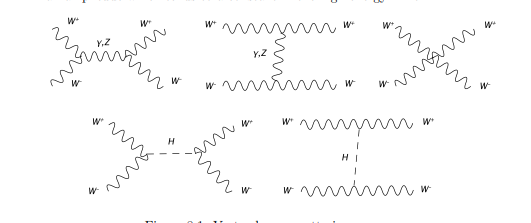
\includegraphics[width=0.8\textwidth]{WW_diagrams_nohiggs.png}
\end{figure}

Following the same formulation of spinor Helicity states taken by Schwarz, and using the $\gamma$ matrices in the Weyl basis $\gamma_{\alpha \dot{\alpha}^{\prime}}^{\mu}=\left(\begin{array}{cc}
0 & \sigma^{\mu \alpha \alpha} \\
\bar{\sigma}_{\alpha \alpha}^{\mu} & 0
\end{array}\right)$
\footnote{Such that, as an example, a scattering amplitude for $e^{+} e^{-} \rightarrow \mu^{+} \mu^{-}$ is $i \mathcal{M}\left(1^{-} 2^{+} 3^{-} 4^{+}\right)=(-i e)^{2}\left\langle 2 \gamma^{\mu} 1\right] \frac{-i g^{\mu \nu}}{s}\left\langle 3 \gamma_{\nu} 4\right]=2 \frac{i e^{2}}{s}[41]\langle 23\rangle$ }

We find the scattering amplitude for the t-channel:
\begin{equation}
    \begin{aligned}
i \mathcal{M}_{t}=&-i g^{2}\left(\frac{\sin^{2}(\theta_w)}{\left(p_{1}-p_{3}\right)^{2}}+\frac{\cos^{2}(\theta_w)}{\left(p_{1}-p_{3}\right)^{2}-m_{Z}^{2}}\right)\left[\left(p_{1}+k_{1}\right)^{\mu} \epsilon\left(p_{1}\right) \cdot \epsilon\left(k_{1}\right)-2 k_{1} \cdot \epsilon\left(p_{1}\right) \epsilon^{\mu}\left(k_{1}\right)-2 p_{1} \cdot \epsilon\left(k_{1}\right) \epsilon^{\mu}\left(p_{1}\right)\right] \\
& \times\left[\left(p_{2}+k_{2}\right)_{\mu} \epsilon\left(p_{2}\right) \cdot \epsilon\left(k_{2}\right)-2 k_{2} \cdot \epsilon\left(p_{2}\right) \epsilon_{\mu}\left(k_{2}\right)-2 p_{2} \cdot \epsilon\left(k_{2}\right) \epsilon_{\mu}\left(p_{2}\right)\right]
\end{aligned}
\end{equation}

The s-channel will have scattering amplitude
\begin{equation}
    \begin{aligned}
i \mathcal{M}_{s}=&-i g^{2}\left(\frac{\sin^{2}(\theta_w)}{\left(p_{1}+p_{2}\right)^{2}}+\frac{\cos^{2}(\theta_w)}{\left(p_{1}+p_{2}\right)^{2}-m_{Z}^{2}}\right)\left[\left(p_{1}-p_{2}\right)^{\mu} \epsilon\left(p_{1}\right) \cdot \epsilon\left(p_{2}\right)+2 p_{2} \cdot \epsilon\left(p_{1}\right) \epsilon^{\mu}\left(p_{2}\right)-2 p_{1} \cdot \epsilon\left(p_{2}\right) \epsilon^{\mu}\left(p_{1}\right)\right] \\
& \times\left[\left(k_{2}-k_{1}\right)_{\mu} \epsilon\left(k_{1}\right) \cdot \epsilon\left(k_{2}\right)-2 k_{2} \cdot \epsilon\left(k_{1}\right) \epsilon_{\mu}\left(k_{2}\right)+2 k_{1} \cdot \epsilon\left(k_{2}\right) \epsilon_{\mu}\left(k_{1}\right)\right]
\end{aligned}
\end{equation}

and the 4-vertex scattering amplitude:
\begin{equation}
    i \mathcal{M}_{4}=i g^{2}\left[2 \epsilon\left(p_{2}\right) \cdot \epsilon\left(k_{1}\right) \epsilon\left(p_{1}\right) \cdot \epsilon\left(k_{2}\right)-\epsilon\left(p_{2}\right) \cdot \epsilon\left(p_{1}\right) \epsilon\left(k_{1}\right) \cdot \epsilon\left(k_{2}\right)-\epsilon\left(p_{2}\right) \cdot \epsilon\left(k_{2}\right) \epsilon\left(p_{1}\right) \cdot \epsilon\left(k_{1}\right)\right]
\end{equation}

Now substituting 
\begin{equation}
    s=\left(p_{1}+p_{2}\right)^{2}, t=\left(p_{1}-p_{3}\right)^{2}
\end{equation}

and the longitudinal polarizations, we get
\begin{equation}
    i \mathcal{M}_{t}=-i \frac{g^{2}}{4 m_{W}^{4}}\left[(s-u) t-3 m_{W}^{2}(s-u)+\frac{8 m_{W}^{2}}{s} u^{2}\right]
\end{equation}

\begin{equation}
    i \mathcal{M}_{s}=-i \frac{g^{2}}{4 m_{W}^{4}}\left[s(t-u)-3 m_{W}^{2}(t-u)\right]
\end{equation}

\begin{equation}
    i \mathcal{M}_{4}=i \frac{g^{2}}{4 m_{W}^{4}}\left[s^{2}+4 s t+t^{2}-4 m_{w}^{2}(s+t)-\frac{8 m_{W}^{2}}{s} u t\right]
\end{equation}

Thus the total total scattering amplitude, assuming no Higgs boson, is the sum of these three amplitudes
\begin{equation}
\begin{aligned}
    i \mathcal{M}_{\text{Total}}^{\text{No Higgs}}(W_{L}^{-} W_{L}^{+} \rightarrow W_{L}^{-} W_{L}^{+}) &= i \mathcal{M}_{t} +i \mathcal{M}_{s} + i \mathcal{M}_{4} \\
    &= -i \frac{g^{2}}{4 m_{W}^{4}} [ (s-u) t-3 m_{W}^{2}(s-u)+\frac{8 m_{W}^{2}}{s} u^{2} + s(t-u)-3 m_{W}^{2}(t-u)\\ & - s^{2} - 4 s t-t^{2}+4 m_{w}^{2}(s+t)+ \frac{8 m_{W}^{2}}{s} u t ] \\
    & \approx -i \frac{g^{2}}{4 m_{W}^{2}} u+\mathcal{O}\left(\left(E / m_{W}\right)^{0}\right)
\end{aligned}
\end{equation}

Notice this problematic high-energy behavior, where the matrix element still grows with energy. Notice also how the strongest high-energy growth, the $E^4$ terms, have been cancelled by summing the diagrams, which is a consequence of gauge-invariance. Nevertheless, we see that the matrix element still grows with energy.


...........................................

 At high energy, an amplitude involving external
longitudinal polarized gauge bosons is equivalent to the amplitude with
the external gauge bosons replaced by the corresponding Goldstone
bosons, up to corrections of order mV /E. At high energy, the
longitudinal guage boson recalls its identity as the Goldstone bosons

------------------------------------
\section{Topological versions}\label{section-topological}

\section{Colorful versions}\label{section-colored}

\section{The structure of Tverberg partitions}\label{section-intersection}

\section{Universal Tverberg partitions}\label{section-universal}

\section{Applications of Tverberg's theorem}\label{section-applications}

\section{Tverberg-type results in distinct settings}\label{section-spaces}

\bibliographystyle{alpha}
\bibliography{references} % see references.bib for bibliography management

\end{document}
